\documentclass[tikz, border=10pt]{standalone}

\usetikzlibrary{arrows}

\begin{document}
	
	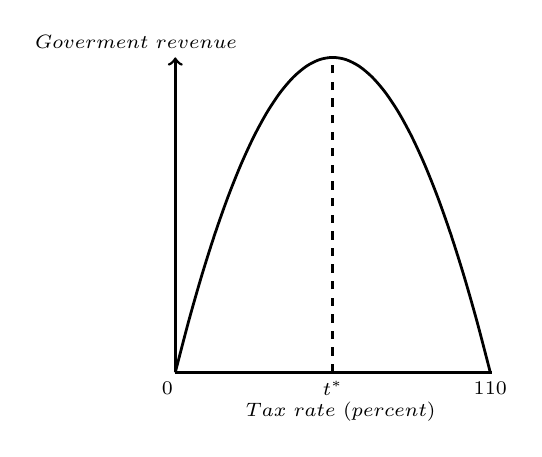
\begin{tikzpicture}[line width=1pt]
		\draw (0, 0) -- (4.02, 0); 	% Горизонтальная линия
		\draw[->] (0, 0) -- (0, 4); % Вертикальная линия
		
		\draw[smooth, domain=0:4] plot(\x,{-((\x)-2)^(2)+4});
		
		\draw[dashed] (2, 0) -- (2, 4); 
		
		\begin{scriptsize}
		\draw (-0.5, 4.2) node {$Goverment~revenue$};
		\draw (2.1, -0.5) node {$Tax~rate~(percent)$};
		
		\draw (-0.1, -0.2) node {$0$};
		\draw (4, -0.2) node {$110$};
		
		\draw (2, -0.2) node {$t^*$};
		\end{scriptsize}
	\end{tikzpicture}
\end{document}